\documentclass[dvipdfmx]{jsarticle}
\usepackage{amsmath,amssymb}
\usepackage[dvipdfmx]{graphicx}
\usepackage{siunitx}
\usepackage{float}
\usepackage{tikz}
\usepackage{circuitikz}
\usepackage{threeparttable}
\graphicspath{{./figure/}}

\begin{document}
\section{目的}

我々が日常的に電力として利用している電気の多くは交流である。
また回路理論を学ぶ上で、交流及び交流回路の基本的な性質の理解は必要不可欠である。
本実験では、以下の3点を理解することを目的とする。

\begin{itemize}
\item
  交流電圧と周波数の測定方法
\item
  交流電圧波形の解析による交流の諸性質
\item
  交流回路における受動素子の構造と働き
\end{itemize}

\section{原理}

\subsection{正弦波交流の表式}

正弦波交流電圧\(v\)や電流\(i\)は次のような数式で表される。

\begin{eqnarray}
v = V_m\sin(\omega t + \theta_v)\\
i = I_m\sin(\omega t + \theta_i)
\end{eqnarray}

ここでは、\(V_m\)は電圧の最大値、\(\theta_v\)は電圧の位相角、\(\theta_i\)は電流の
位相角、\(t\)は時間\(\omega\)は角周波数を表す。
また、角周波数\(\omega\)と周期\(T\)、周波数\(f\)の関係は次のような式で表される。

\begin{equation}
\omega = \frac{2}{\pi} = 2\pi f[\rm rad/s]
\end{equation}

\subsubsection{瞬時値と実効値}

ある時刻の交流の大きさを瞬時値と言う。実効値は、瞬時値の2乗を1周期の間平均した
値の平方根として定義され、交流の大きさを表すときに使われる。
実効値の物理的な意味は、「交流電圧(電流)を抵抗に加えたときに消費する電力が、
その実効値と同じ大きさの直流電圧(電流)を加えたときの消費電力と等しくなる。」
ということである。 実効値は次の式で求められる。

\begin{eqnarray}
V = \frac{V_m}{\sqrt{2}}, I = \frac{I_m}{\sqrt2}
\end{eqnarray}

\subsection{各種計測器で測定可能な電気的諸量}

本実験で使用する計測器で測定できる電気量を表\ref{tb:table_dennki}に示す。

\begin{table}[h]
  \caption{各種計測器で測定可能な電気的諸量}
  \label{tb:table_dennki}
  \begin{threeparttable}
    \begin{tabular}{|c|c|c|c|c|c|}\hline 
      \multicolumn{2}{|c|}{電気量} & アナログ回路計 & ディジタルマルチメータ & 交流電子電圧計 & オシロスコープ \\ \hline
      \multicolumn{2}{|c|}{抵抗} & ○\footnotemark[2] & ◎\footnotemark[1] & ×\footnotemark[4] & × \\ \cline{1-6}
      直流 & 電圧 & ○ & ◎ & × & △\footnotemark[3]\\ \cline{2-6}
       & 電流 & ○ & ◎ & × & ×\\ \hline
      交流 & 電圧 & ○ & ○ & ◎ & △\\ \cline{2-6}
       & 電流 & ○ & ○ & × & ×\\ \hline
      \multicolumn{2}{|c|}{周波数} & × & ◎ & × & △\\ \hline
      \multicolumn{2}{|c|}{波形} & ×  & ×  & ×  & ◎ \\ \hline 
    \end{tabular}
    \begin{tablenotes}\footnotesize
      \item[1] 優
      \item[2] 良
      \item[3] 可
      \item[4] 不可
      \end{tablenotes}
\end{threeparttable}
\end{table}
\subsection{リサジュー図形を用いた位相差の測定}

リサジュー図形とは互いに直行する単振動が平面上に描く軌跡である。互いに直行する単振動を

\begin{eqnarray}
  x(t) = A_1\sin(\omega_1 t + \theta_1) \\
	y(t) = A_2\sin(\omega_2 t + \theta_2) 
\end{eqnarray}

とする時、点$(x(t), y(t))を様々なtの値に対して、X-Y平面上$
でプロットして得られる図形がリサジュー図形である。

$x(t)とy(t)$の周波数が等しい場合、リサジュー図形を用いて位相差を求めることができる。

\begin{eqnarray}
  |\sin(\theta_1 - \theta_2)| = \sin^{-1} \frac{b}{a}
\end{eqnarray}

$a$は$x軸方向$の最大値と最小値の差、$b$は$y(t) = 0$を満たす2点の距離である。

\subsection{円筒形コイルのインダクタンスと測定方法}
絶縁された電線を円筒形に一重に巻くことによって作られたコイルのインダクタンス$L$は
次式で与えられる。

\begin{eqnarray}
  L = K \frac{\pi^2 D^2 N^2}{l} \times 10^{-7}
\end{eqnarray}

$Dは直径、lは長さ、Nは巻き数、Kは長岡係数である。$長岡係数とは、直径と長さの比$D/l$で決まる
定数である。

\begin{figure}[h]
  \centering
  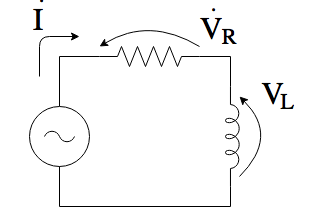
\includegraphics[scale=0.4]{RL_Series_Circut.png}
  \caption{RL直列回路}
  \label{fig:RL_Series_Circuit}
\end{figure}

図\ref{fig:RL_Series_Circuit}に示す
RL直列回路において電圧$\dot V_R, \dot V_L$の実効値(または最大値)と角周波数$\omega、抵抗R$
からインダクタンス$L$を以下の式から求める事ができる。

\begin{eqnarray}
  L = \frac{R}{\omega}\frac{|\dot V_R|}{|\dot V_L|}
\end{eqnarray}

\subsection{平行平板コンデンサのキャパシタンスと測定方法}
同じ形の2枚の金属板を平行に配置する事によって作られた平行平板コンデンサのキャパシタンス
$C$は次式で与えられる。

\begin{eqnarray}
  C = \epsilon_0 \epsilon_r \frac{S}{d}
\end{eqnarray}

$\epsilon_0は真空中の誘電率、\epsilon_rは金属板間を満たす物質の比誘電率、Sは金属板の
面積、dは金属板間の距離である。$

\begin{figure}[h]
  \centering
  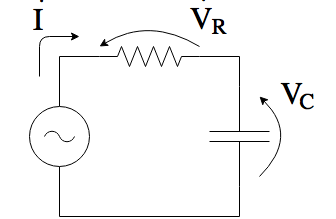
\includegraphics[scale=0.4]{RC_Series_Circuit.png}
  \caption{RC直列回路}
  \label{fig:RC_Series_Circuit}
\end{figure}

図\ref{fig:RC_Series_Circuit}に示すRC直列回路において、電圧$\dot V_R, \dot V_C$の実効値(または最大値)と角周波数$\omega、抵抗R$
から、キャパシタンス$C$を以下の式から求めることができる。

\begin{eqnarray}
  C = \frac{1}{\omega R} \frac{|\dot V_R|}{|\dot V_C|}
\end{eqnarray}

\section{実験方法}
\subsection{各種計測器による交流電圧の測定}
以下の手順に従って、図に示す回路において各種計測器を用いて交流電圧を測定した。
\begin{itemize}
  \item [(1)]ブレッドボードを用いて、図の回路を作製せよ。
  \item [(2)]オシロスコープで図中の電圧$v$を測定し、オシロスコープに表示される
            電圧の最大値が3 [V]、周波数が1 [kHz]になるように発振器の出力を調節する。
  \item [(3)]電圧$v$が測定できるように、交流電子電圧計を回路につなぎ、計測値が2[V]に
              なるよう発振器の電圧ツマミを調節する。
  \item [(4)](3)の状態での各種計測器による電圧測定値を表に記録する。
  \item [(5)]発振器の周波数を調整してオシロスコープの周波数表示が表に示す値になるようにし、
            各周波数における電圧を表に示す計測器で測定する。この実験では、発振器の電圧調整ツマミは
            (4)の状態から変化させない。
\end{itemize}
\subsection{オシロスコープを用いた交流電圧の取得}
\subsubsection{測定データの取得}
前の実験「各種計測器による交流電圧の測定」(3)の状態にする。オシロスコープを
用いて測定データを保存する。また、表に実験に使用した抵抗の抵抗値と周波数を示す。
\subsubsection{測定データの利用}
\begin{itemize}
  \item [(1)]表計算ソフトウェアを用いて保存された.cvsファイルを開き、.xlsxファイルとして保存する。
  \item [(2)]表計算ソフトウェアの機能を用いて、オシロスコープで測定されたデータから、電圧波形のグラフを作成する。
            グラフは、横軸を時間、縦軸を電圧とする。
\end{itemize}
\subsection{表計算ソフトウェアを用いた交流の解析}
第3.2節で取得したデータを用いて、表計算ソフトウェア上で以下の解析を行う。
\begin{itemize}
  \item [(1)]データ保存時に交流電子電圧計で測定した測定値(実効値)を記録する。
        またその電圧値から、計算によって電圧の最大値と半周期分の平均値、及び
        電流の実効値を求め、記録する。
  \item [(2)]測定データから周期、周波数を求める。
  \item [(3)]半周気分の瞬時値から、最大値と平均値を求め、記録する。
  \item [(4)]半周期文の瞬時電圧値の一つ一つの値を表で記録した抵抗値で除算する事により、半周期分の瞬時電流値を求める。
  \item [(5)]電圧と電流の瞬時値から、半周期に渡っての電力の瞬時値を求める。
  \item [(6)]前項の瞬時電圧の半周期分の平均値を求め、記録する。また、求めた電力の平均値
            が、実行電圧値と実行電流値の積と等しくなることを確認する。
\end{itemize}
\subsection{瞬時電圧を表す式の導出と比較}
以下の手順に従って、測定データから瞬時電圧を表す式を求め、式から計算される
電圧値と測定値を比較する。
\begin{itemize}
  \item [(1)]第4.2節でオシロスコープで保存したデータから求めた周波数から、角周波数$\omega$を求める。
  \item [(2)]瞬時電圧の式$v(t) = V_m \sin(\omega t + \theta)$に前項の$\omega$を代入し、
              測定された交流電圧の瞬時値を表す式を求める。ただし$\theta = 0$とする。
  \item[(3)]列挙した時刻における位相$\omega t$を以下の式から求める事ができる。
  \item[(4)]各時刻における瞬時電圧値を、(2)で求めた式を用いて算出する。また、計算値と測定値を比較する。
\end{itemize}
\subsection{位相差の測定}
\begin{itemize}
  \item [(1)]図に示す回路を作製する
  \item [(2)]図中の電圧$V, V_1, V_2$をオシロスコープで測定し、データを保存する。
  \item [(3)](2)で保存したデータから、各電圧の最大と周波数を求める。
  \item [(4)]$VとV_1、VとV_2、V_1とV_2の組み合わせについて$、以下の二通りの方法で位相差を測定する。
    \begin{description}
      \item [正弦波の時間差から求める]正弦波が同じ位相になる点の時間差$\delta t$から位相差$\phi = \omega \delta t$を求める事ができる。
      \item [リサジュー図形から求める]リサジュー図形を用いて、2.3の原理に基づき位相差を求める。
    \end{description}
  \item[(5)]求めた各値から、各電圧の瞬時値を与える式を求める。ただし、位相角$\theta$はゼロとし、$V$を基準とし$V_1, V_2$の位相角を決定する。
\end{itemize}
\subsection{インダクタンスの作成と測定}
\subsubsection{コイルの作製}
直径7.5 [cm]の塩化ビニル製のパイプとフォルマル線を用いて、25巻と50巻の二種類のコイルを作製する。
\subsubsection{インダクタンスの測定}
作製したコイルの内、25巻のものを$L_1$、50巻のものを$L_2$とする。
以下の四つの場合において、図\ref{fig:RL_Series_Circuit}のRL直列回路をブレッドボード上に作製し、
$|\dot V_R|, |\dot V_L|$を測定する。ただし、周波数は100 [kHz]、抵抗Rは$100 [\Omega]$とする。
\begin{itemize}
  \item [(1)]$L_1$のみ
  \item [(2)]$L_2$のみ
  \item [(3)]$L_1, L_2$の直列接続
  \item [(4)]$L_1, L_2$の並列接続
\end{itemize}
\subsection{キャパシタンスの制作と測定}
\subsubsection{コンデンサの作製}
アルミホイル、OHPシート、両面テープを用いて、極板の形状が5 [cm] $\times$ 5 [cm]と
10 [cm] $\times$ 5 [cm]の二種類のコンデンサを作製する。
\subsubsection{キャパシタンスの測定}
作製したコンデンサの内、極板形状が5 [cm] $\times$ 5 [cm]のものを$C_1$、
10 [cm] $\times$ 5 [cm]のものを$C_2$とする。
以下の四つの場合において、図\ref{fig:RC_Series_Circuit}のRC直列回路をブレッドボード上に作製し、
$|\dot V_R|, |\dot V_C|$を測定する。ただし、周波数は1 [kHz]、抵抗Rは500 $[k\Omega]$とする。
\begin{itemize}
  \item [(1)]$C_1$のみ
  \item [(2)]$C_2$のみ
  \item [(3)]$C_1, C_2$の直列接続
  \item [(4)]$C_1, C_2$の並列接続
\end{itemize}
\end{document}